\documentclass[uplatex]{jsarticle}
\usepackage{UCLabZemiReport}

%%%%%%%%%%%%%%%%%%%%%%%%%%%%%%%%
%          ヘッダ情報          %
%%%%%%%%%%%%%%%%%%%%%%%%%%%%%%%%
\year{2019}				% 年度(4桁の西暦)
\MemberID{000}			% メンバーID(3桁).連絡網参照
\DocumentNo{001}		% ドキュメントNo.(3桁の連番)
\date{2019/04/23}		% 報告会日(YYYY/MM/DD のフォーマットで)
\author{鈴木 秀和}		% 報告者氏名(姓名の間に半角スペース)

% 報告会名称(作成するドキュメントに応じて切替)
\MeetingName{第1回ゼミ報告会}	        % 学部生の通常ゼミ
%\MeetingName{第1回大学院ゼミ報告会}	% 修士の通常ゼミ

\makeheader		% ヘッダ・フッタを表示するコマンド(消さない!!)


\begin{document}		% ここから下に報告内容を記述する

%%%%%%%%%%%%%%%%%%%%%%%%%%%%%%%%
%        アブストラクト        %
%%%%%%%%%%%%%%%%%%%%%%%%%%%%%%%%
% アブストラクト:報告内容を完結に書く(行った内容とその結果) 

\begin{abstract}
ここに報告内容を簡潔にまとめたアブストラクトを記述する.
何を行って,何が分かったのか,何が問題となっているのか等.
\end{abstract}


%%%%%%%%%%%%%%%%%%%%%%%%%%%%%%%%
%             本文             %
%%%%%%%%%%%%%%%%%%%%%%%%%%%%%%%%
% 本文:実施内容,結果,課題,今後の予定などを章節を設定して記述する.

\section{はじめに}

卒業研究などにおけるゼミでは,本テンプレートを利用してゼミレポートを作成する.
本ファイルを複製して,本文の内容を修正して作成すればよい.

\LaTeX を用いてゼミレポートを作成する際の注意事項について述べる.


\section{ファイル構成}

ゼミレポートキットには,以下のファイルが含まれている.

\begin{enumerate}
\item \texttt{main.tex}:\\
\LaTeX ファイル.
このファイルを\textbf{複製}して,それに報告内容を記述すればよい.
なお,コピーしたファイルの名前を「(各自のメンバーID)-(ドキュメントID).tex」に変更する.
ヘッダに記載されるDocument No. 以降の文字列が該当する.
このサンプルでは「000-001.tex」になる.
%
\item \texttt{main.pdf}:\\
\texttt{main.tex}から生成したPDFファイル.
%
\item \texttt{UCLabZemiReport.sty}:\\
ゼミレポート用スタイルファイル.
フォーマットに関する変更がない限り,特に編集する必要はない.
%
\item \texttt{reference.bib}:\\
文献データが管理されたファイル.
\LaTeX ファイルの1つ上の階層のディレクトリに配置する.
%
\item \texttt{main.bbl}:\\
\texttt{reference.bib}ファイルをコンパイルして生成された文献リスト.
このファイルが\LaTeX 文章に読み込まれて表示される.
%
\item \texttt{ZemiReport.bst}:\\
参考文献の出力フォーマットを定義したスタイルファイル.
情報処理学会のテンプレート\texttt{ipsjunsrt.bst}をUTF-8化し,一部修正を加えている.
\LaTeX ファイルの1つ上の階層のディレクトリに配置する.
%\part{title}
\item 各種画像ファイル:\\
掲載する図の画像ファイル.
\end{enumerate}


\section{テンプレートの使い方}

\subsection{ヘッダ・フッタ}

ヘッダに記載される情報は,本\LaTeX ファイルの9〜18行目に設定する.
\begin{itemize}
\item \verb|\year{年度}|:年度を4桁の西暦で入力する.
%
\item \verb|\MemberID{メンバーID}|:3桁の研究室メンバーIDを入力する.
メンバーIDは研究室名簿(連絡網)から確認できる.
メンバーIDが3桁に満たない場合は,0を付けて3桁にする(例:5 $\rightarrow$ 005).
%
\item \verb|\DocumentNo{ドキュメントNo.}|:ドキュメントNo.は,B4のゼミからこれまでに作成した報告書の通算番号である.
すなわち,ある回の報告会で報告書を作成しなかった場合でも,次回の報告書では\underline{必ず連番となる}.
大学院へ進学した場合も引き続き連番とする.
報告会名称(\verb|\MeetingName{報告会名称}|)が異なる場合は,ドキュメントNo.をそれぞれの報告会ごとに管理する.
%
\item \verb|\date{報告日}|:報告会が行われる日付を,``\texttt{YYYY/MM/DD}''のフォーマットで入力する.
%
\item \verb|\author{報告者氏名}|:報告者の氏名を入力する.
なお,姓と名の間には半角スペースを入力すること.
%
\item \verb|\MeetingName{報告会名称}|:報告会の名称を回数と併せて入力する.(例:第1回卒業研究報告会)

\end{itemize}

上記値を設定したら,\verb|\makeheader|でヘッダ・フッタの出力を行う(\LaTeX ファイルの19行目).

\subsection{見出し(章節)}
章を設定する場合は\verb|\section|,節を設定する場合は\verb|\subsection|,項を設定する場合は\verb|\subsubsection|を用いる.

\subsection{フォント}
\LaTeX で文章を作成する場合,フォントは考慮する必要はない.
スタイルファイルで定義されており,本文は明朝体となっている.

\subsubsection{句読点}
句点は「,」(カンマ),読点は「.」(ピリオド)に統一する.
Windowsではタスクバー右にある入力(「A」や「あ」と表示されているボタン) $\to$ プロパティ $\to$ 詳細設定から規定値を設定できる.

\subsubsection{全角文字と半角文字}
和文は全角,英数字記号は半角で入力する.
もちろん,\LaTeX コマンドは半角で入力すること.

\subsubsection{太文字・下線}
指定文字列を{\bf 太文字}にする場合は,\verb|{\bf 文字列}|のように記述する.
なお,太字にするとフォントが明朝体からゴシック体に変更される.

指定文字列に\underline{下線}を引く場合は,\verb|\underline{文字列}|のように記述する.

\subsubsection{等幅フォント}
コマンドや変数などを記載する場合は等幅フォントにする.
\verb|\texttt{}|コマンドで括弧内の文字列が等幅フォント(Courier系)に変更される.

\subsubsection{ダブル引用符}
「``」および「''」はダブル引用符キーで入力するのではなく,シングル引用符を2回続けて入力する.
例えば左ダブル引用符の場合,左シングル引用符「\texttt{`}」を連続で入力すると,「``」と表示される.
右ダブル引用符の場合,右シングル引用符「\texttt{'}」を連続で入力すると,「''」と表示される.

\subsubsection{\LaTeX ファイルにおけるコメント化}
「\%」記号を入力すれば,そこから後ろの部分がコメント化される.
なお,「\%」記号を直接入力したい場合は「\verb|\%|」と入力する.

\subsection{箇条書き}
\subsubsection{単純箇条書き}
\verb|itemize|環境を用いる.
項目は\verb|\item|コマンドを用いて設定する.
\begin{itemize}
\item 箇条書き項目1
\item 箇条書き項目2
\end{itemize}

\subsubsection{列挙型箇条書き}
\verb|enumerate|環境を用いる.
\begin{enumerate}
\item 箇条書き項目1
\item 箇条書き項目2
\end{enumerate}
%
また,\verb|\begin{enumerate}[I.]|のように箇条の数値部分のスタイルを指定することができる.
(\texttt{A},\texttt{a},\texttt{I},\texttt{i}等.\texttt{1)}のように括弧なども設定できる)
\begin{enumerate}[I.]
\item 箇条書き項目3
\item 箇条書き項目4
\end{enumerate}

\subsubsection{見出し付箇条書き}
\verb|description|環境を用いる.
見出しの後に改行したい場合は,単純に\verb|\\|するのではなく,\verb|\mbox{}\\|とする.
\begin{description}
\item[見出し1:] 改行しない箇条書き項目
\item[見出し2:]\mbox{}\\
改行した箇条書き項目
\end{description}

\subsection{脚注}
脚注をつけたい場合は,本文中に\verb|\footnote|コマンドを挿入し\footnote{ここに脚注文章を入力する.},その中に脚注部分に表示したい文章を記入する.

\subsection{図・表}
研究室wikiを参考にして図表を挿入する.
なお,図表番号の参照には\verb|\ref|コマンドではなく,情報処理学会テンプレートにて使われている\verb|\figref|と\verb|\tabref|コマンドを用いる.
これにより,「図」や「表」の文字を別途記入する必要はない.
例えば\figref{fig:NetConf}や\tabref{tab:NetworkLab}のように用いる.
表の文字サイズを本文より小さくするために,\verb|\begin{tabular}|コマンドの直前に\verb|\small|コマンドを記述する.


\subsubsection{図が一つの場合}
figフォルダ内にfigure1.pdfがあるならば,\figref{fig:NetConf}のように挿入できる.

\verb|\begin{figure}[h]|における\texttt{[h]}は,挿入場所を示す.
必要に応じ,下記のいずれかを使用する.
特に,学会発表における原稿や論文は\texttt{[t]}か\texttt{[b]}で図表の位置をドキュメントの上下に揃えること.
なお,2段組みの原稿などでは,\verb|\begin{figure*}[t]|のように,アスタリスクをつけることで,横幅一杯に図を張り付けすることができる.


\begin{itemize}
	\item \texttt{[h]}:コマンドの位置に図を挿入.報告書はこれで良い.here
	\item \texttt{[t]}:ドキュメントの上部に図を挿入.top
	\item \texttt{[b]}:ドキュメントの下部に図を挿入.bottom
\end{itemize}


\verb|\begin{center}|は中央ぞろいにする.

\verb|\includegraphics|は実際に図を挿入するコマンドである.
\texttt{width=}で幅を指定する.
この幅は,\verb|\columnwidth|オプションを基準値とし,割合を示している.
主なオプションは以下の通り.
本文が2段組みの原稿などで使用すれば違いがわかる.
なお,図解すると\figref{fig:tex-margin}\footnote{引用:TeXメモ:\url{http://www.slis.tsukuba.ac.jp/~fujisawa.makoto.fu/cgi-bin/wiki/index.php?TeX%A5%E1%A5%E2#p61e1b46}}のようになる.

\verb|\caption|はキャプションを示す.


\verb|\label|はTexソース内で参照する際に利用する.
\verb|{}|がそのままラベルとなる.
図は「\texttt{fig:XXX}」,表は「\texttt{tab:XXX}」,ソースコードは「\texttt{src:XXX}」など,どのラベルかすぐに把握できるように管理するとよい.


\begin{itemize}
	\item \verb|\columnwidth|:column,つまり列の長さを基準とする.
	2段組みのテキストでは1つの段落の長さが基準となる.
	\item \verb|\textwidth|:ドキュメントに記載される本文の幅一杯を基準とする.おそらくほとんど使わない.
\end{itemize}



\begin{figure}[ht]
	\begin{center}
		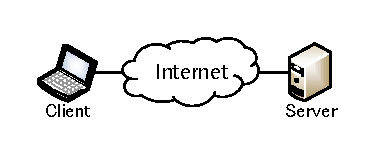
\includegraphics[width=0.4 \columnwidth]{fig/figure1.pdf}
		\caption{ネットワーク構成}
		\label{fig:NetConf}
	\end{center}
\end{figure}


\begin{figure}[ht]
	\begin{center}
		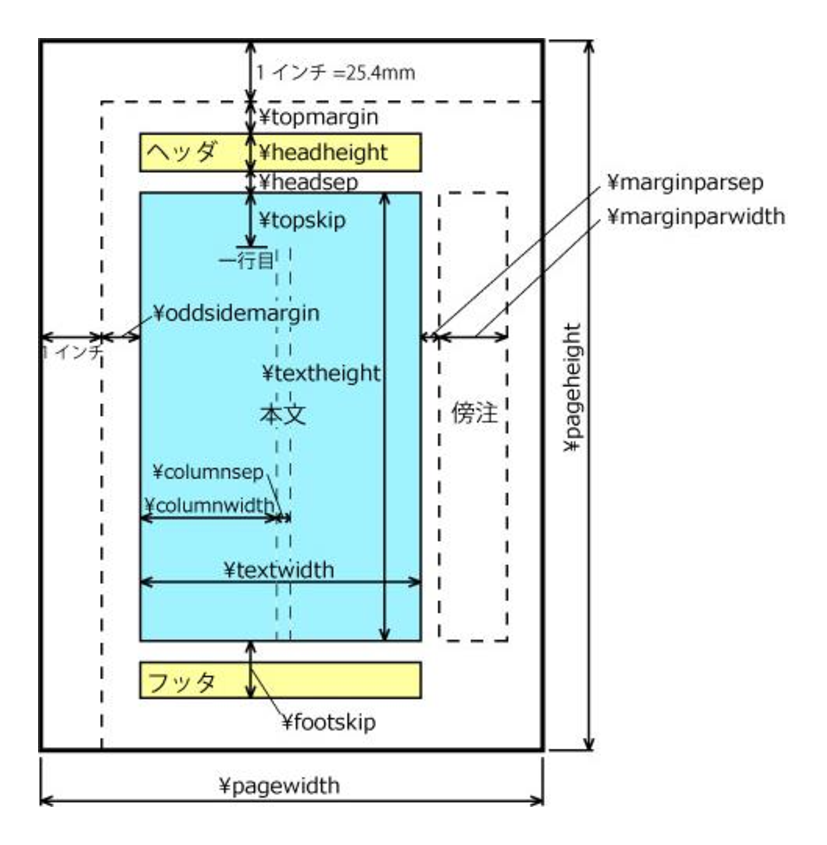
\includegraphics[width=0.51 \columnwidth]{fig/tex-margin.pdf}
		\caption{2段組みのドキュメントにおける各長さの解説}
		\label{fig:tex-margin}
	\end{center}
\end{figure}



\subsubsection{図を並べる場合}
\verb|\begin{minipage}|コマンドを使うことにより,\figref{fig:figure1-2-1}や\figref{fig:figure1-2-2}に示すように図を並べられる.

\verb|\begin{minipage}|コマンドにより2つ以上の図や票を並べられる.
可読性の観点から2つまでにするとよい.
サイズの指定はテキスト幅\verb|\textwidth|の割合を指定するが,合計が1.0にならないようにする
\footnote{例では0.49と0.49の\verb|\minipage|環境を作成している.サイズの合計が1.0になると,図が横方向に並んで配置されず,縦方向に並んでしまう.}.

\verb|\begin{minipage}|コマンドの場所を示すオプションは,図を並べる場合\verb|[b]|,表を並べる場合\verb|[t]|,図と表を並べる場合\verb|[h]|にするとキャプションの位置がそろい,きれいに見える.

\verb|\caption|コマンドを\verb|\minipage|コマンドの外に記述することにより,\figref{fig:figure1-3}のように複数の図に対して一つのキャプションを割り当てられる\footnote{\figref{fig:figure1-3}では\verb|\figure|に対してキャプションを割り当てている.一方,\figref{fig:figure1-2-1}や\figref{fig:figure1-2-2}では\verb|\minipage|に対してキャプションを割り当てている.}.
写真を並べるときに活用できる.


\begin{figure}[ht]
	\centering
	\begin{minipage}[b]{0.49\textwidth}    % b にするとキャプションの位置が揃ってきれい
		\centering
		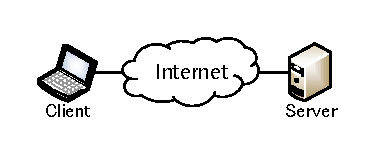
\includegraphics[width=1 \columnwidth]{fig/figure1.pdf}
		\caption{図を並べる場合(その1)}
		\label{fig:figure1-2-1}
	\end{minipage}
	%
	\begin{minipage}[b]{0.49\textwidth}
		\centering
		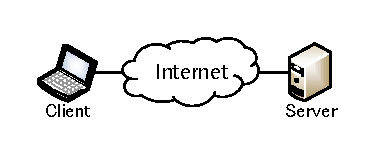
\includegraphics[width=1 \columnwidth]{fig/figure1.pdf}
		\caption{図を並べる場合(その2)}
		\label{fig:figure1-2-2}
	\end{minipage}
\end{figure}


\begin{figure}[ht]
	\centering
	\begin{minipage}[b]{0.49\textwidth}    % b にするとキャプションの位置が揃ってきれい
		\centering
		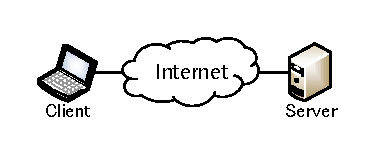
\includegraphics[width=1 \columnwidth]{fig/figure1.pdf}
	\end{minipage}
	%
	\begin{minipage}[b]{0.49\textwidth}
		\centering
		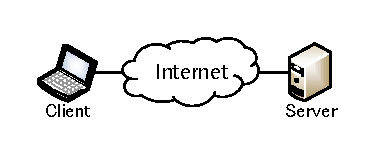
\includegraphics[width=1 \columnwidth]{fig/figure1.pdf}
	\end{minipage}
	\caption{キャプションを一つで図を並べる(写真向け)}
	\label{fig:figure1-3}
\end{figure}

\subsubsection{表を挿入する場合}
\verb|\begin{table}|を用いることで,\tabref{tab:NetworkLab}のように表を挿入できる.

\verb|\begin{tabular}{lll}|コマンドでは,表の中身を記す.
\verb|{lll}|は文字列の整列を指定している.
\texttt{|}(縦線)記号により,縦線を引ける.
見出しとデータを切り分ける際に使用する.
整列記号には,下記がある.

\begin{itemize}
	\item l:左揃い
	\item r:右揃い
	\item c:中央ぞろい
	\item p\{10zw\}:指定した長さである10zw\footnote{zwは全角文字1文字分の横幅を示す.zhでは全角文字1文字分の高さを示す.}分の長さを上限にし,オーバーした分は自動改行する.
\end{itemize}

\verb|\hline|コマンドは,水平に罫線を引くコマンドである.
罫線の場所は,情報処理学会のテンプレに沿う.
表の見出しの上は2本,見出しの下は1本,表の一番下の行の下に1本引く.
表の行ごとにデータを記載し,データは\verb|&|記号で区切る.
また,最も右の列で必ず\verb|\\|記号により改行する.

表にキャプションを設定する場合,\verb|\begin{threeparttable}|環境内に\verb|\begin{tablenotes}|環境を作ることで挿入できる.
表内に\verb|\tnote|で脚注番号を指定し,\verb|\begin{tablenotes}|内で\verb|\item[脚注番号]|により記述する.

\begin{table}[ht]
 \centering
 \caption{通信系研究室}
 \label{tab:NetworkLab}
 \small	% 表中の文字サイズを小さくする.
 \begin{threeparttable}	% 脚注環境
  \begin{tabular}{lll}
  \hline\hline
  教員 & 研究室名 & 部屋番号 \\
  \hline
  渡邊 晃 & 情報ネットワーク & 2-414-2 \\
  宇佐見 庄五 & 情報通信方式 & 2-414-3 \\
  旭 健作 & 情報通信システム & 2-305 \\
  鈴木 秀和 & ユビキタスコンピューティング \tnote{1} & 2-414-1 \\
  \hline
  \end{tabular} 
  \begin{tablenotes}\footnotesize  % \tnote{} と \item[] で脚注
  % 下記パッケージを追加する必要がある
  % \usepackage{threeparttable} % 表の下に脚注を追加
  \item[1] UCLab.本研究室.
  \end{tablenotes}
 \end{threeparttable}
\end{table}

\subsubsection{図と表を並べる場合}
\verb|\begin{minipage}|を使えば図と表を並べることもできる.
ただし,図表のカウントを意識する必要がある.
\LaTeX では,図1, 図2, ...などの図表のカウントは\verb|\begin{figure}|もしくは\verb|\begin{table}|環境内の\verb|\caption|コマンドが入力されたタイミングでカウントアップされる.
\verb|\begin{figure}|環境内で\verb|\begin{tabular}|環境を作ることで表を挿入できるものの,\verb|\caption|コマンドを入力すると\texttt{figure}がカウントアップされてしまう.
そこで,\verb|\begin{minipage}|環境内で\verb|\makeatletter|,\verb|\def\@captype{table}|,\verb|\makeatother|コマンドを入力することで,そのminipage内の\verb|\caption|コマンドによるカウントアップが\verb|\def\@captype{table}|で指定したものになる.
これにより,\tabref{tab:para-tab},\figref{fig:para-fig}のように正しいキャプション番号で図表を並べることができる.
352-354行目あたりを消してコンパイルしてみるとすぐにわかる.

\begin{figure}[ht]
	\centering
	\begin{minipage}[h]{0.47 \textwidth}
		% table を挿入するうため,ここで一工夫
		\makeatletter               % この3行が必要
		\def\@captype{table}      % この行でキャプションを table に変更
		\makeatother
		\caption{横幅一杯の表}
		\label{tab:para-tab}
		\begin{threeparttable}
			%  
			\begin{tabular*}{\hsize}{ll}   
			% {tabular*}{\hsize}で横幅一杯の表にできる
				\hline \hline
				cl1 & cl2 \tnote{1} \\
				\hline
				S1 & R1 \\
				\hline
			\end{tabular*}
			\begin{tablenotes}\footnotesize
				\item[1] footnote comment.
			\end{tablenotes}
		\end{threeparttable}
	\end{minipage}
	%
	\begin{minipage}[h]{0.49 \textwidth}
		% figure環境なので,普通に図を挿入
		\centering
		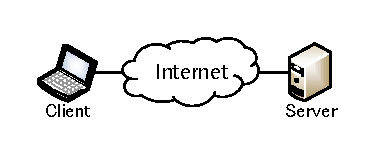
\includegraphics[width=1 \linewidth]{fig/figure1.pdf}
		\caption{cap fig}
		\label{fig:para-fig}
	\end{minipage}
\end{figure}


\subsection{マクロの活用}

\verb|\begin{figure}|コマンドなど,覚えるのは大事だが毎回入力するのは効率が悪い.
そこで,TexStudioのマクロ機能を使えばShiftキーとFキーで任意のコマンドを呼び出せる.
マクロ$\to$マクロを編集から設定できる.
ただし,デフォルトの設定では,Shift + F3キーはべつの機能がある.
その場合は,オプション$\to$キーボードショートカット$\to$メニュー$\to$マクロからキー割り当てを変更する.


\subsection{参考文献}
参考文献は\BibTeX により作成する.
文章に記載したい文献情報を\texttt{reference.bib}に記述する.
TexStudioのデフォルトでは,ビルド時(ショートカットキー:F1)に,自動で\LaTeX 文章と同じ名前で拡張子が\texttt{.bll}の文献リストファイルが生成され,参照される.
\texttt{.bll}のみを生成する場合,ツール$\to$文献,もしくはF8を押す.
コンパイル時に同時実行させないようにするには,オプションを開き,高度な設定を表示にした後,ビルド$\to$ビルドオプション$\to$コンパイル前に参考文献を確認・更新のチェックを外す.
ただし,本文中で文献を参照していない場合,bblファイルは生成されない.

\subsubsection{参考文献リスト(拡張子:.bib)}
bibファイルに文献データを記載する.

文献管理にMendeleyを利用している場合は,必要な文献(または全て)を選択し,MendeleyのメニューからFile$\rightarrow$Exportを選択すれば,bibファイルとしてエクスポートできる.
必要であれば,bibファイルをエディタで開いて,必要な項目の追加や不要な項目の削除など,直接編集すればよい.

なお,Mendelayでbibファイルをエクスポートした場合,bibファイルの一部を修正する必要がある.
そこで,JabRef\footnote{http://jabref.sourceforge.net/}というスタンドアロン型文献管理アプリケーションを利用する.
JabRefによりbibファイルを開いたら,姓と名の間にカンマがあるので,それを削除する(姓と名の間の半角スペースはそのまま残す).
削除し忘れると,\LaTeX 文章に読み込んだ際に姓と名が逆順で表示されてしまう.
また,URLの項目がある場合は削除する.
これは通常の論文・研究報告などの学会発表の文献についてはURLを掲載しないためである.
URLを掲載するのは,Webページを参照した場合のみでよい.

\subsubsection{参考文献の参照}
本文中で文献を参照する場合は,\verb|\cite{CiteKey}|を用いる\cite{GSRA-Proxy}.
\texttt{CiteKey}の部分には,各自が文献データに設定したラベルとする.
設定されたラベルは,bibファイルの各文献データの先頭行,またはbblファイルの\verb|\bibitem|の直後に記載されている.
複数の文献を一度に参照する場合は\verb|\cite|コマンドで複数のラベルを記述すればよい\cite{IdLocatorTransport,Android80221Handover}.

\subsubsection{参考文献リストファイル(拡張子:.bbl)}
研究報告書に掲載する参考文献には,文献の発表機関を掲載する必要がある.
この場合,bibファイルからbblファイルが生成された後,エディタによりbblファイルを開く.
``\texttt{author}''に記載していた著者名が記載されているので,手作業で著者名の後ろに``(機関名)''を追記する
\footnote{機関名はできるかぎり略記する.(例:名古屋大学 $\rightarrow$ 名大,慶應義塾大学 $\rightarrow$ 慶大,情報通信研究機構 $\rightarrow$ NICT,etc.)}.
なお,情報工学科の関係者が発表した文献については,``(名城大)''と記載しなくてもよい.


\section{おわりに}
必ず報告会では\LaTeX 文章を用いて報告書を作成するように.
また,常日頃の関連研究の調査で発見した文献をMendeleyなどで管理し,bibファイルを容易に作成できるよう心がけてほしい.


%%%%%%%%%%%%%%%%%%%%%%%%%%%%%%%%
%           参考文献           %
%%%%%%%%%%%%%%%%%%%%%%%%%%%%%%%%
% .texファイルから見た各ファイルの相対パスを設定する
\bibliographystyle{UCLabZemiReport}	% UCLabZemiReport.bst
\bibliography{reference}		    % reference.bib


%%%%%%%%%%%%%%%%%%%%%%%%%%%%%%%%
%             付録             %
%%%%%%%%%%%%%%%%%%%%%%%%%%%%%%%%
\appendix
\section{更新履歴}
\begin{enumerate}
\item 2011/04/27
\begin{itemize}
\item 初版作成.
\end{itemize}
%
\item 2011/05/06
\begin{itemize}
\item 不具合を修正?
\end{itemize}
%
\item 2012/04/04
\begin{itemize}
\item プリアンブルに「MeetingName(報告会名称)」のパラメータを追加し,どの種類の報告会資料かわかるようにヘッダに反映.報告会回数もここに含めるようにする.
\item 上記に伴い,プリアンブルから「MeetingNo(報告会回数)」のパラメータを削除.
\item ヘッダの報告者氏名の前に,研究室名が表記されるように修正.
\end{itemize}
%
\item 2017/03/21
\begin{itemize}
	\item TexLiveとTexStudioの環境に合わせる(platex $\to$ uplatex)
	\item eps図の説明消去.PDF図に統一.
	\item ソースコードの記載方法を追加(jlistingの追加)
	\item 図表の挿入方法に追記
	\item TexStudioのマクロについて記載
\end{itemize}
%
\item 2019/04/23
\begin{itemize}
	\item 報告会名称を変更
	\item \verb|\verb|コマンドの一部を\verb|\texttt|コマンドに変更
\end{itemize}
%
\end{enumerate}

\end{document}